% Created 2018-11-18 dom 20:30
% Intended LaTeX compiler: pdflatex
\documentclass[xcolor={usenames,svgnames,dvipsnames}]{beamer}
\usepackage[utf8]{inputenc}
\usepackage[T1]{fontenc}
\usepackage{graphicx}
\usepackage{grffile}
\usepackage{longtable}
\usepackage{wrapfig}
\usepackage{rotating}
\usepackage[normalem]{ulem}
\usepackage{amsmath}
\usepackage{textcomp}
\usepackage{amssymb}
\usepackage{capt-of}
\usepackage{hyperref}
\usepackage{color}
\usepackage{listings}
\usepackage{mathpazo}
\usepackage{gensymb}
\usepackage{amsmath}
\usepackage{chemarr}%flechas para reacciones químicas (SFER.tex)
\bibliographystyle{plain}
\AtBeginSubsection[]{\begin{frame}[plain]\tableofcontents[currentsubsection,sectionstyle=show/shaded,subsectionstyle=show/shaded/hide]\end{frame}}
\AtBeginSection[]{\begin{frame}[plain]\tableofcontents[currentsection,hideallsubsections]\end{frame}}
\usepackage[emulate=units]{siunitx}
\sisetup{fraction=nice, decimalsymbol=comma, retain-unity-mantissa = false}
\newunit{\wattpeak}{Wp}
\newunit{\watthour}{Wh}
\newunit{\amperehour}{Ah}
\usepackage{steinmetz}
\hypersetup{colorlinks=true, linkcolor=Blue, urlcolor=Blue}
\renewcommand{\thefootnote}{\fnsymbol{footnote}}
\beamertemplatenavigationsymbolsempty
\setbeamertemplate{footline}[frame number]
\setbeamercolor{alerted text}{fg=blue!50!black} \setbeamerfont{alerted text}{series=\bfseries}
\usetheme[hideothersubsections]{Goettingen}
\usecolortheme{rose}
\usefonttheme{serif}
\author{Oscar Perpiñán Lamigueiro}
\date{\url{http://oscarperpinan.github.io}}
\title{Energía Solar Fotovoltaica}
\subtitle{Aplicaciones y Contexto Mundial}
\hypersetup{
 pdfauthor={Oscar Perpiñán Lamigueiro},
 pdftitle={Energía Solar Fotovoltaica},
 pdfkeywords={},
 pdfsubject={},
 pdfcreator={Emacs 25.2.2 (Org mode 9.1.13)}, 
 pdflang={Spanish}}
\begin{document}

\maketitle

\section{Aplicaciones de la Energía Solar Fotovoltaica}
\label{sec:org05381b2}

\subsection{Clasificación}
\label{sec:org7e41953}

\begin{frame}[label={sec:orgf1463f2}]{Definición}
\begin{itemize}
\item Un sistema fotovoltaico es el conjunto de equipos eléctricos y
electrónicos que producen energía eléctrica a partir de la radiación
solar.

\item El principal componente de este sistema es el módulo fotovoltaico.

\item El resto de equipos incluidos en un sistema fotovoltaico depende de la aplicación.
\end{itemize}

\begin{block}{Tipos}
\begin{itemize}
\item Conectados a red (\emph{grid connected})

\item Autónomos (\emph{off-grid})

\item Bombeo
\end{itemize}
\end{block}
\end{frame}

\begin{frame}[label={sec:org739aeeb}]{}
\begin{center}
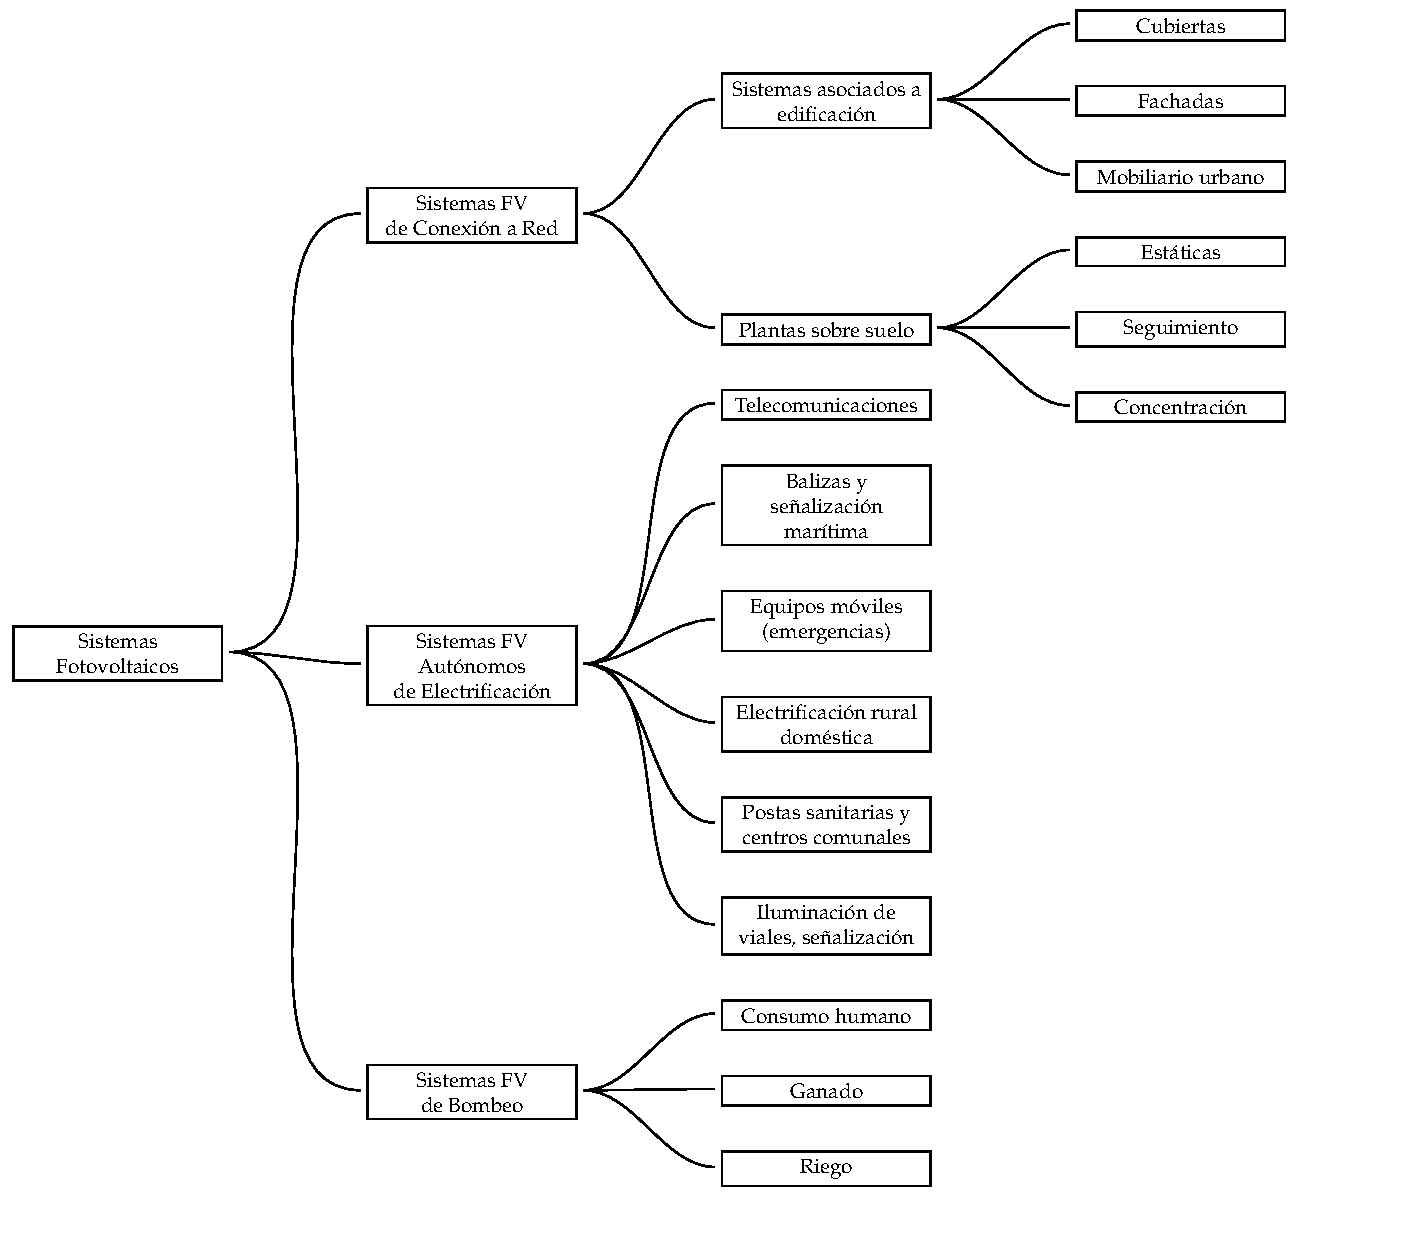
\includegraphics[width=.9\linewidth]{../figs/ClasificacionSistemas.pdf}
\end{center}
\end{frame}

\subsection{SFCR}
\label{sec:orgb2bb065}

\begin{frame}[label={sec:org16858e2}]{Definición}
\begin{itemize}
\item Los sistemas conectados a red producen energía eléctrica para ser
\alert{inyectada en la red convencional}.

\item Dado que no deben satisfacer ninguna demanda de consumo de forma
directa ni garantizar el mismo, \alert{no necesitan incorporar equipos de
acumulación de energía}.

\item Para permitir el correcto acoplamiento con la red eléctrica estos
sistemas \alert{incorporan un equipo inversor} que adecúa la potencia
producida por el generador fotovoltaico a las condiciones de la red
convencional.
\end{itemize}
\end{frame}

\begin{frame}[label={sec:orgd6d5d5f}]{Tipos de SFCR}
\begin{block}{Sistemas sobre Suelo}
\begin{itemize}
\item Concebidos exclusivamente para producir energía y obtener el
rendimiento económico asociado. Suelen superar los
\(\SI{100}{\kilo\watt}\) de potencia.
\end{itemize}
\end{block}

\begin{block}{Sistemas en Edificación}
\begin{itemize}
\item Abarcan funciones adicionales a la producción de energía, tales como
sustitución de componentes arquitectónicos, efecto estético,
sombreado de acristalamientos, etc.

\item En general, son sistemas más pequeños que los instalados sobre
suelo, normalmente de potencias inferiores a los
\(\SI{100}{\kilo\watt}\).
\end{itemize}
\end{block}
\end{frame}

\begin{frame}[label={sec:orgf66ffb1}]{Sistemas sobre Suelo}
\begin{center}
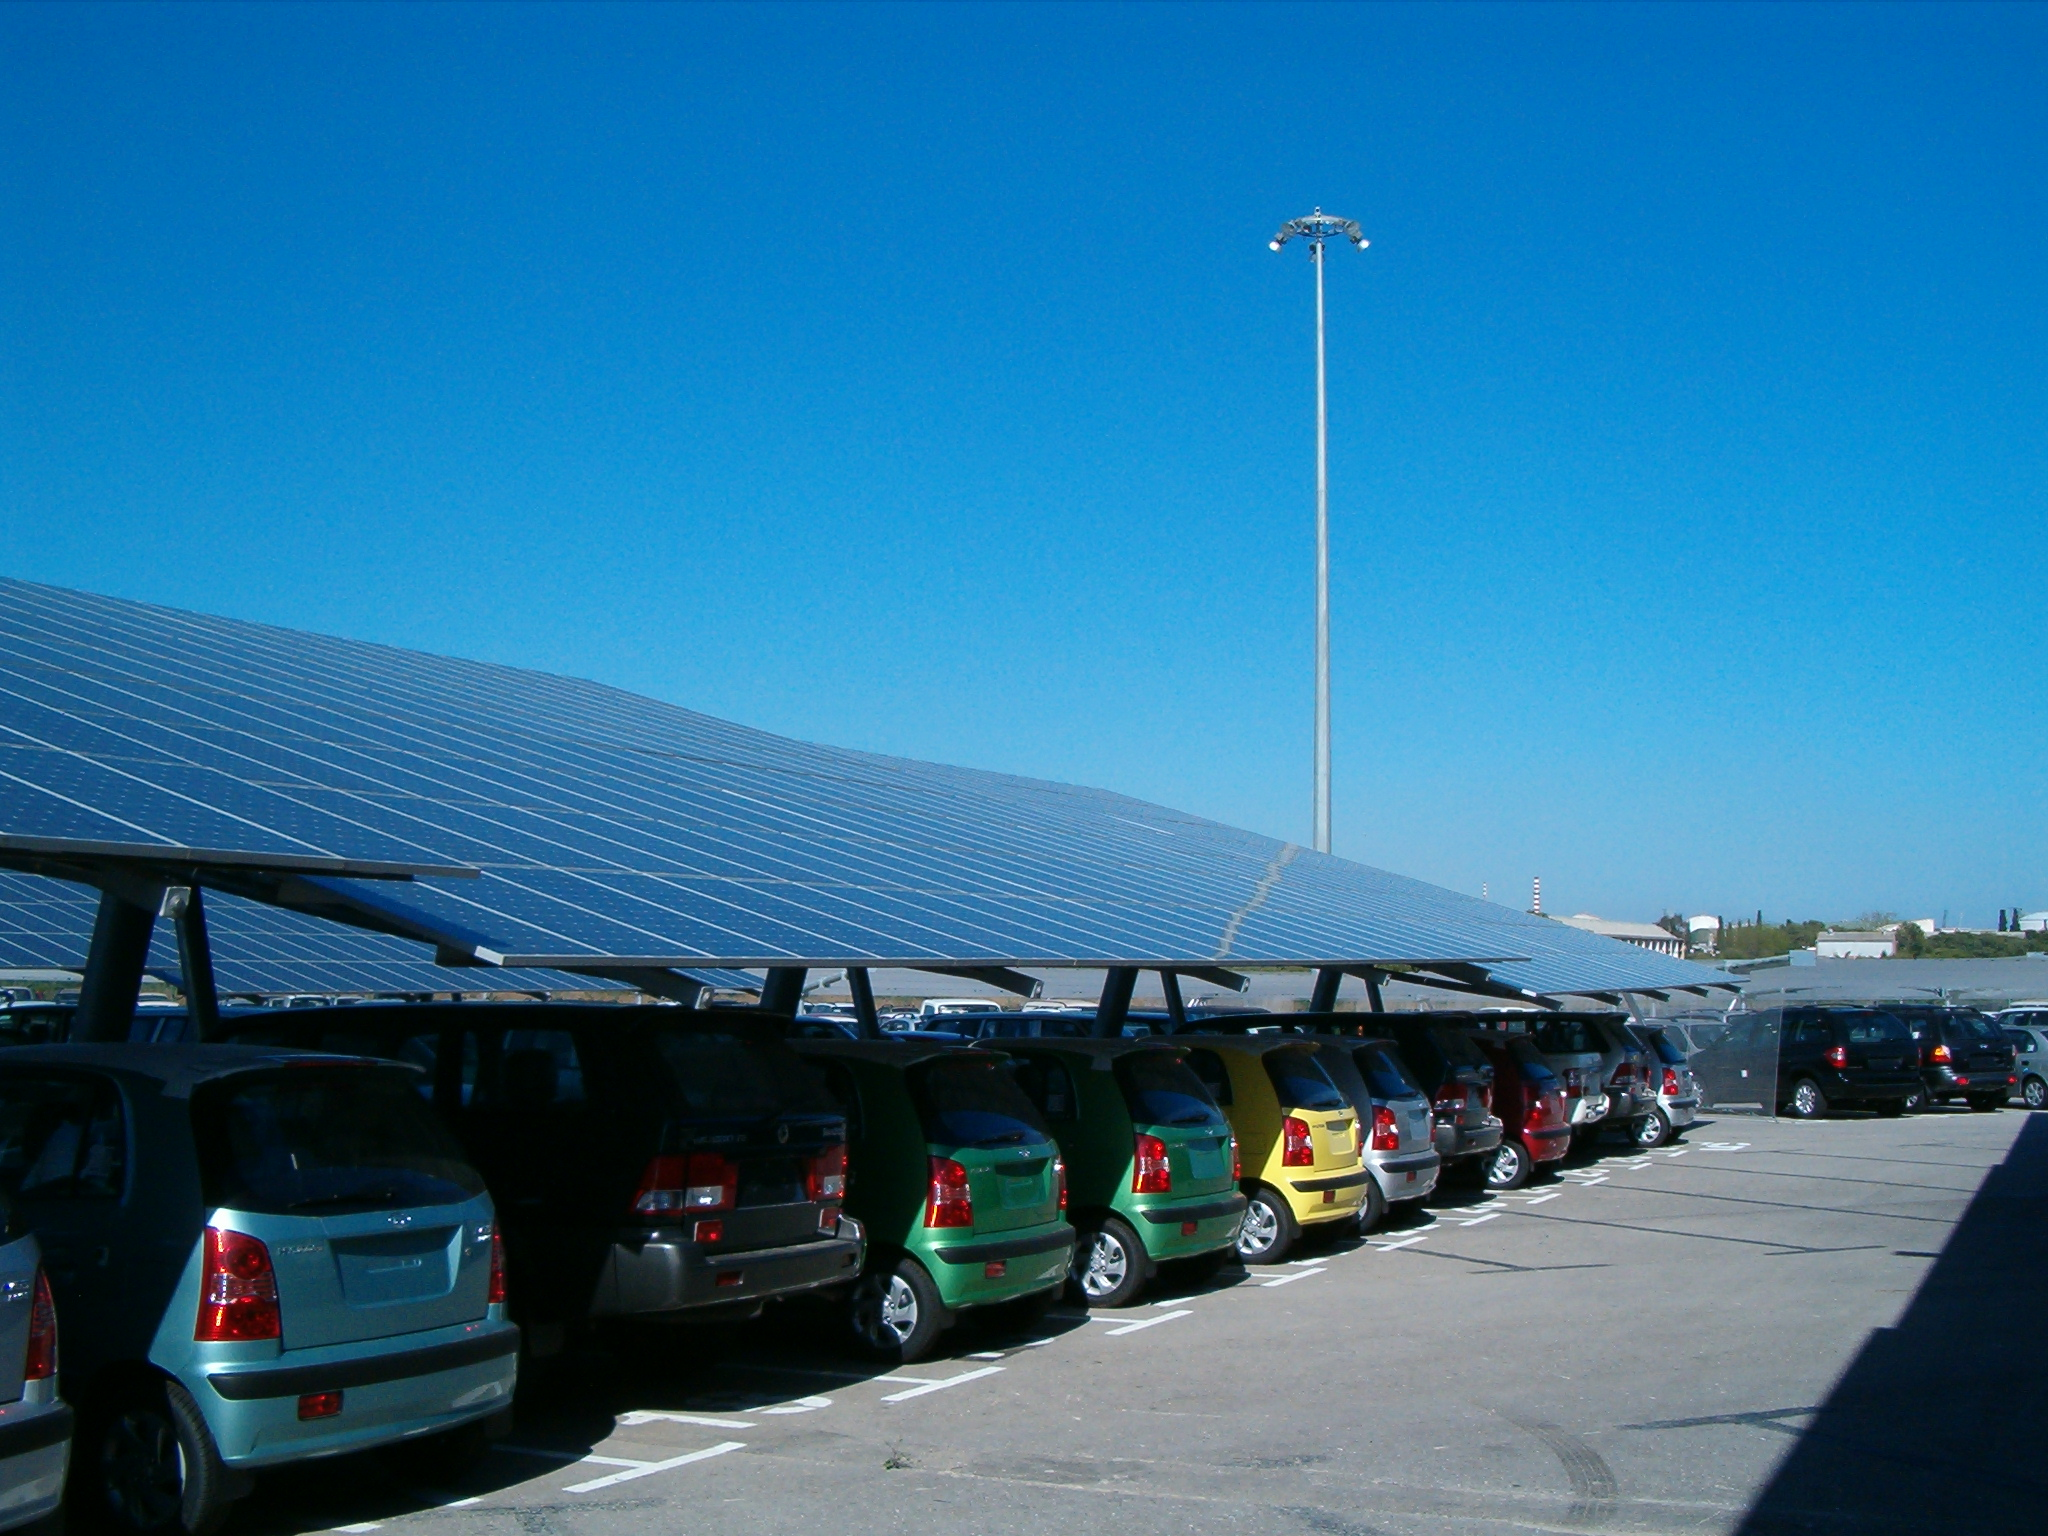
\includegraphics[width=.9\linewidth]{../figs/Photocampa.jpg}
\end{center}
\end{frame}

\begin{frame}[label={sec:org2c41945}]{Sistemas en Edificación}
\begin{center}
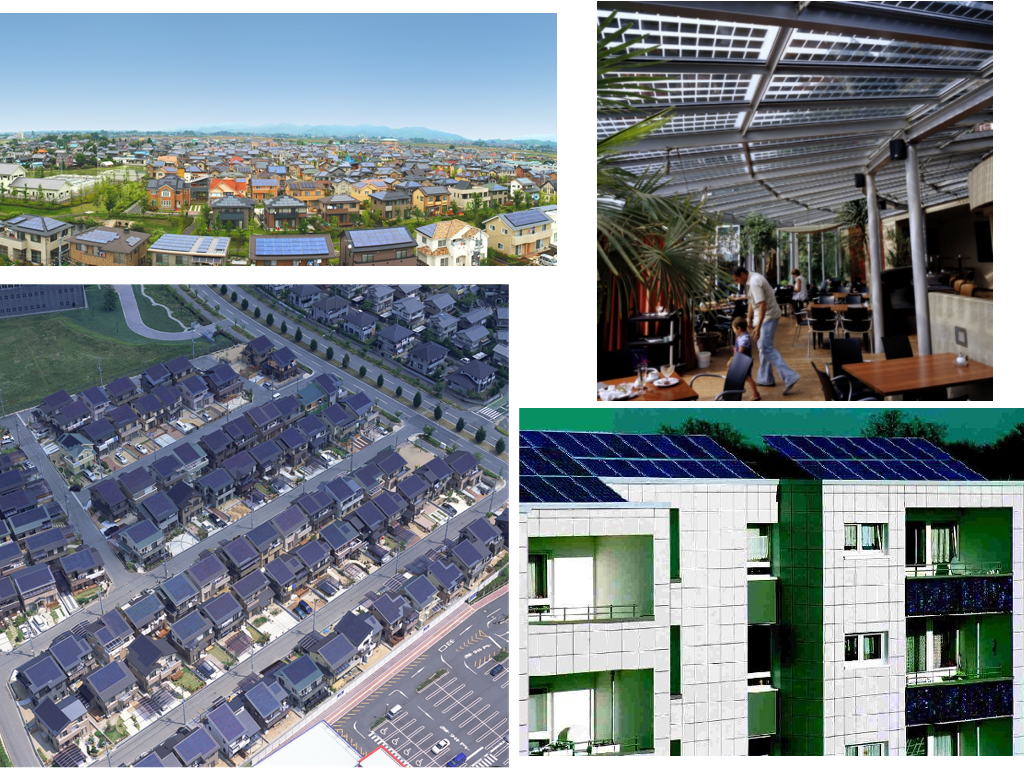
\includegraphics[width=.9\linewidth]{../figs/PVUrban.png}
\end{center}
\end{frame}

\subsection{Sistemas Autónomos}
\label{sec:orgdbc0c75}
\begin{frame}[label={sec:orgc9ff61a}]{Definición}
\begin{itemize}
\item Objetivo: satisfacer una demanda energética determinada.

\item Incorporan un equipo de acumulación de energía.

\item Tipos: profesionales, electrificación rural y pequeño consumo.
\end{itemize}
\end{frame}

\begin{frame}[label={sec:org0a46d98}]{Aplicaciones profesionales}
\begin{itemize}
\item Radioenlaces, la protección catódica de gasoductos, hoteles, señales
de tráfico y navegación aérea, refrigeración de vacunas, equipos
remotos de adquisición y transmisión de datos, e incluso
alimentación de equipos espaciales como satélites.

\item Requieren una fiabilidad muy elevada.

\item El corte de suministro en estas aplicaciones tiene consecuencias de
elevado coste: generador fotovoltaico y un acumulador electroquímico
de tamaño superior al estrictamente necesario para reducir al mínimo
la probabilidad de fallo.

\item En algunos casos se opta por incorporar un grupo electrógeno, ya sea
para reducir el tamaño del acumulador o para funcionar como equipo
de socorro.
\end{itemize}
\end{frame}

\begin{frame}[label={sec:orgf905f06}]{}
\begin{center}
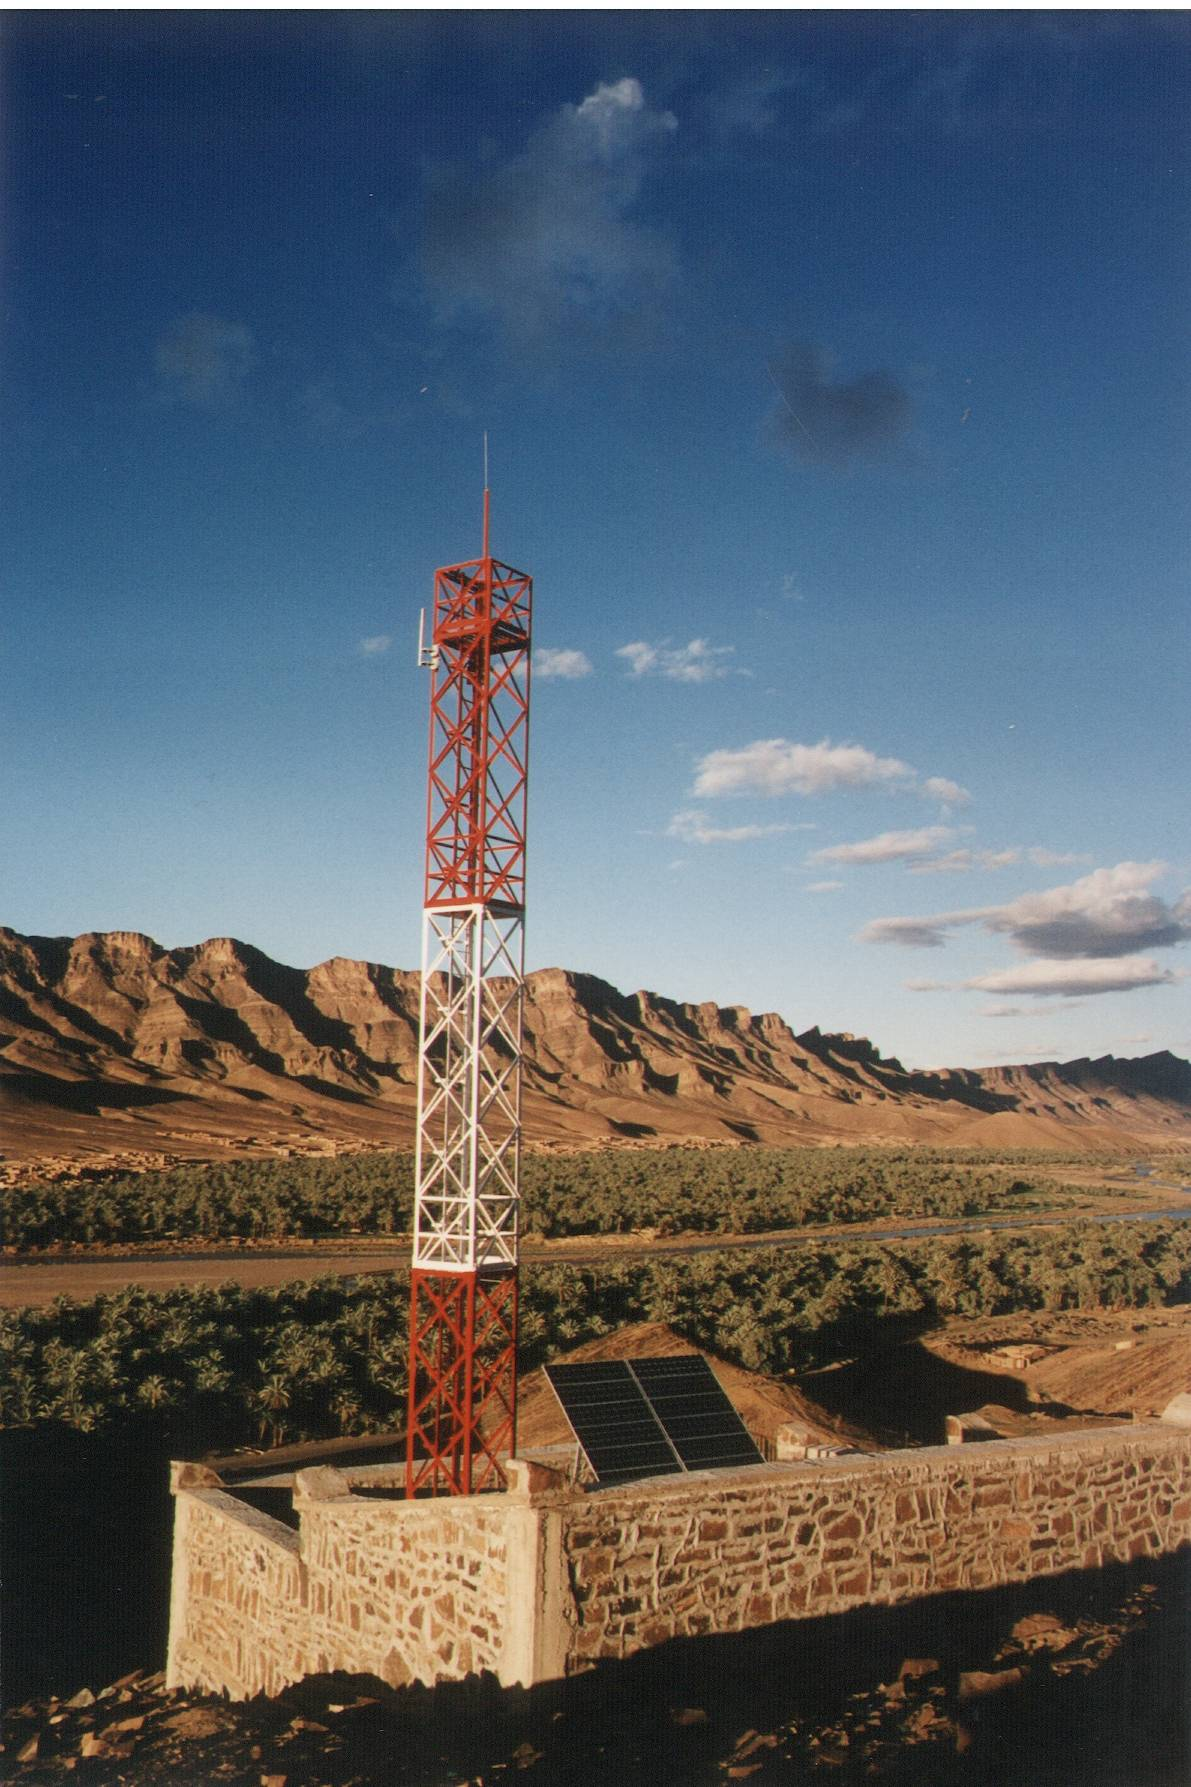
\includegraphics[height=0.95\textheight]{../figs/TelefoniaRural.jpg}
\end{center}
\end{frame}

\begin{frame}[label={sec:orgfebfb3c}]{Sistemas de Electrificación Rural}
\begin{itemize}
\item Los sistemas de electrificación rural suministran energía eléctrica
a poblaciones rurales alejadas de redes eléctricas convencionales.

\item Proporcionan energía para alimentar equipos de iluminación, radio,
televisión y pequeñas herramientas eléctricas.

\item Son sistemas frecuentemente englobados en programas de cooperación
al desarrollo, financiados por ONG's u organismos como el Banco
Mundial o la Unión Europea.

\item Dentro de los sistemas de electrificación rural predominan los
sistemas domésticos (\emph{solar home systems, SHS}) y las centrales
híbridas.
\end{itemize}
\end{frame}

\begin{frame}[label={sec:orgd2fee76}]{SHS}
\begin{itemize}
\item Los sistemas domésticos habitualmente con potencias de
\(\SI{100}{\watt}\) o \(\SI{200}{\watt}\), están asociados a una
vivienda familiar y en algunos casos a centros comunales o centros
de salud.
\end{itemize}

\begin{center}
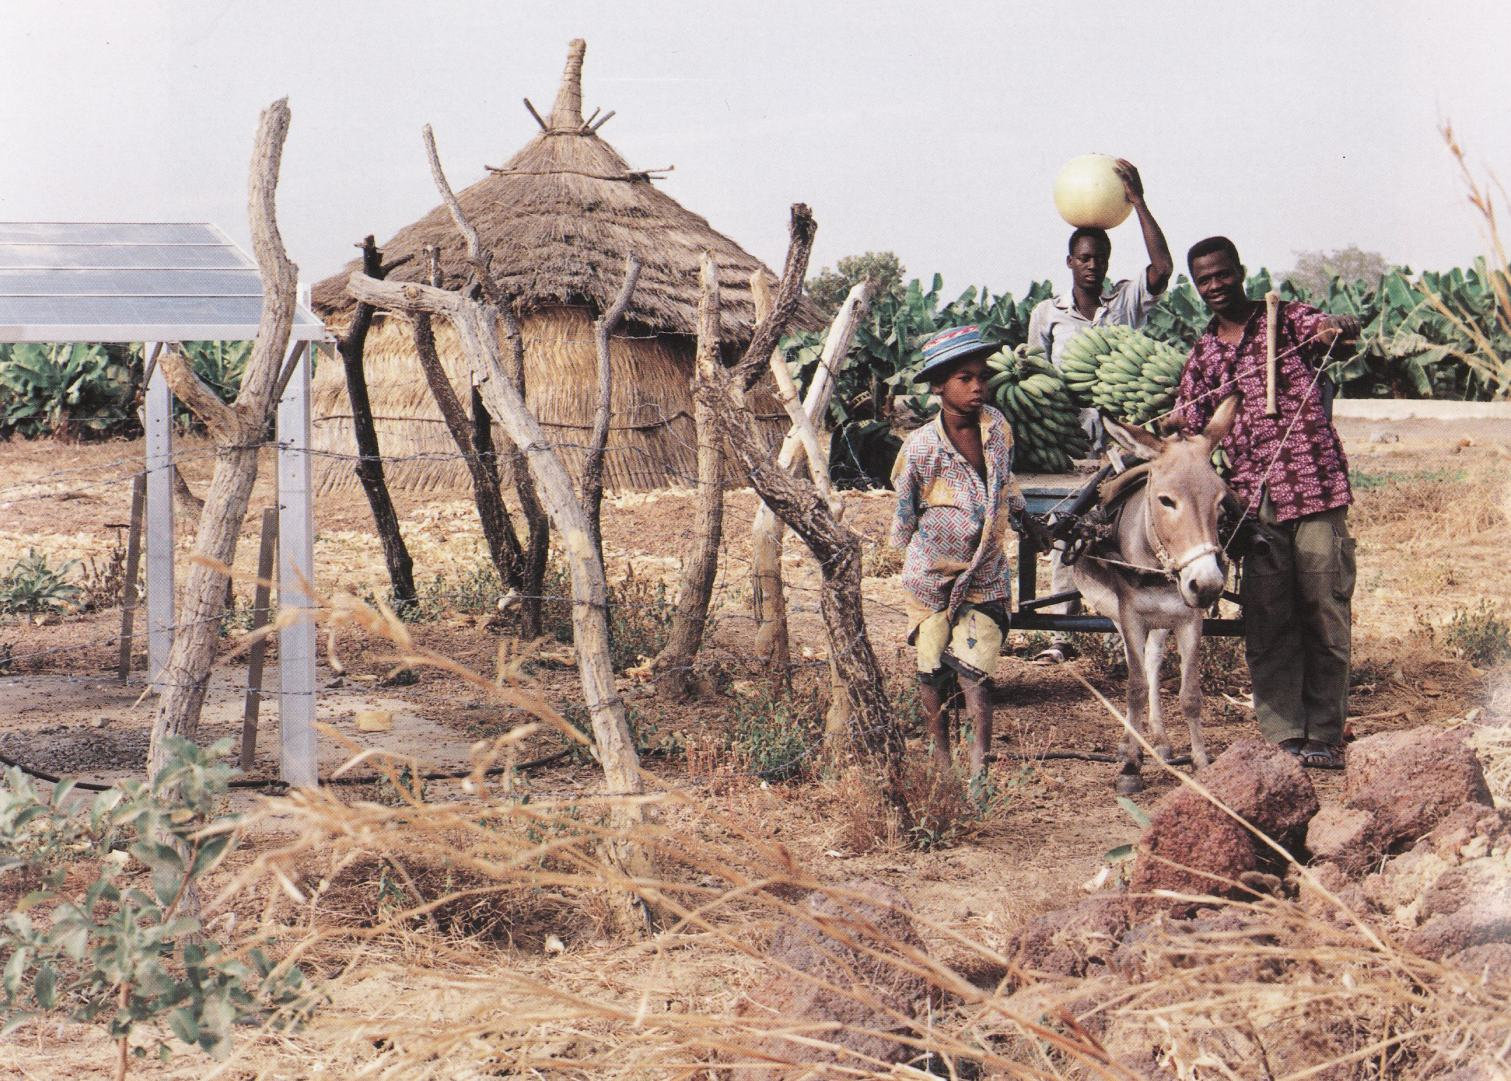
\includegraphics[width=.9\linewidth]{../figs/er.jpg}
\end{center}
\end{frame}


\begin{frame}[label={sec:org22e9f34}]{Híbridos}
\begin{itemize}
\item Las centrales híbridas, compuestas por un generador fotovoltaico, un
acumulador electroquímico y un grupo electrógeno o turbina eólica,
proveen una red eléctrica para un poblado rural.

\item El tamaño de estas centrales depende del tamaño de la población
asociada, con potencias que van desde los \(\SI{10}{\kilo\watt}\)
hasta los \(\SI{100}{\kilo\watt}\).
\end{itemize}
\end{frame}

\begin{frame}[label={sec:org0a9119f}]{Aplicaciones pequeño consumo}
Pequeños módulos fotovoltaicos, frecuentemente de silicio amorfo,
alimentando equipos electrónicos como calculadoras o relojes,
cargadores de móviles, pequeñas herramientas eléctricas, balizas
domésticas, etc.
\end{frame}


\subsection{Sistemas de Bombeo}
\label{sec:org470f15a}
\begin{frame}[label={sec:org103b81e}]{Definición}
\begin{itemize}
\item Los sistemas de bombeo emplean la energía eléctrica que produce el
generador fotovoltaico para accionar una motobomba que eleva y
transporta agua desde un acuífero hasta un depósito o una red de
distribución.

\item Para reducir costes y aumentar la fiabilidad es frecuente acumular
la energía en forma de energía potencial del agua almacenada en el
depósito elevado.

\item Suministro de agua para consumo humano o animal, el riego de
plantaciones individuales o comunitarias y la desalinización del
agua extraída con sistemas de ósmosis inversa.
\end{itemize}
\end{frame}
\begin{frame}[label={sec:org03323a6}]{}
\begin{center}
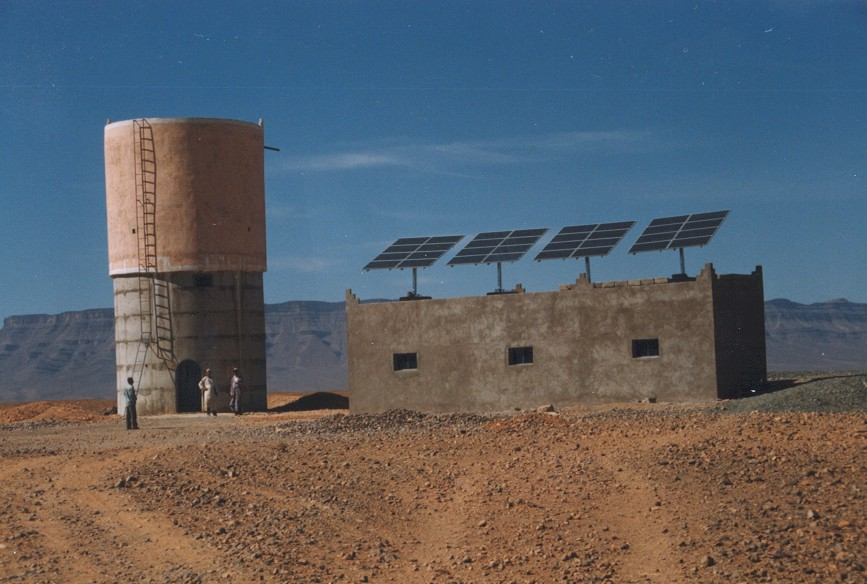
\includegraphics[width=.9\linewidth]{../figs/Bombeo.jpg}
\end{center}
\end{frame}

\section{Contexto Mundial}
\label{sec:org006c4e6}

\subsection{Mercado Fotovoltaico}
\label{sec:orgfe65e2d}

\begin{frame}[label={sec:org461f095}]{Potencia Instalada}
Según el informe del mercado fotovoltaico publicado por la Agencia
Internacional de la Energía (IEA-PVPS)\footnote{\url{http://www.iea-pvps.org/fileadmin/dam/public/report/statistics/IEA-PVPS\_-\_A\_Snapshot\_of\_Global\_PV\_-\_1992-2017.pdf}}, a finales de 2017 había una
potencia fotovoltaica acumulada de \SI{402.5}{\giga\watt} a nivel
mundial.
\end{frame}

\begin{frame}[label={sec:org702a348}]{Potencia por Países}
\begin{block}{29 países han superado la cifra de \SI{1}{\giga\watt} de potencia instalada acumulada}
\begin{enumerate}
\item China: \SI{131}{\giga\watt}
\item Estados Unidos \SI{51}{\giga\watt}
\item Japón: \SI{49}{\giga\watt}
\item Alemania: \SI{42}{\giga\watt}
\item Italia: \SI{19.7}{\giga\watt}
\item India: \SI{18.3}{\giga\watt}
\item Reino Unido: \SI{12.7}{\giga\watt}
\item Francia: \SI{8}{\giga\watt}
\item Australia: \SI{7.2}{\giga\watt}
\item España: \SI{5.6}{\giga\watt}
\end{enumerate}
\end{block}
\end{frame}

\begin{frame}[label={sec:org01d15cf}]{}
\begin{center}
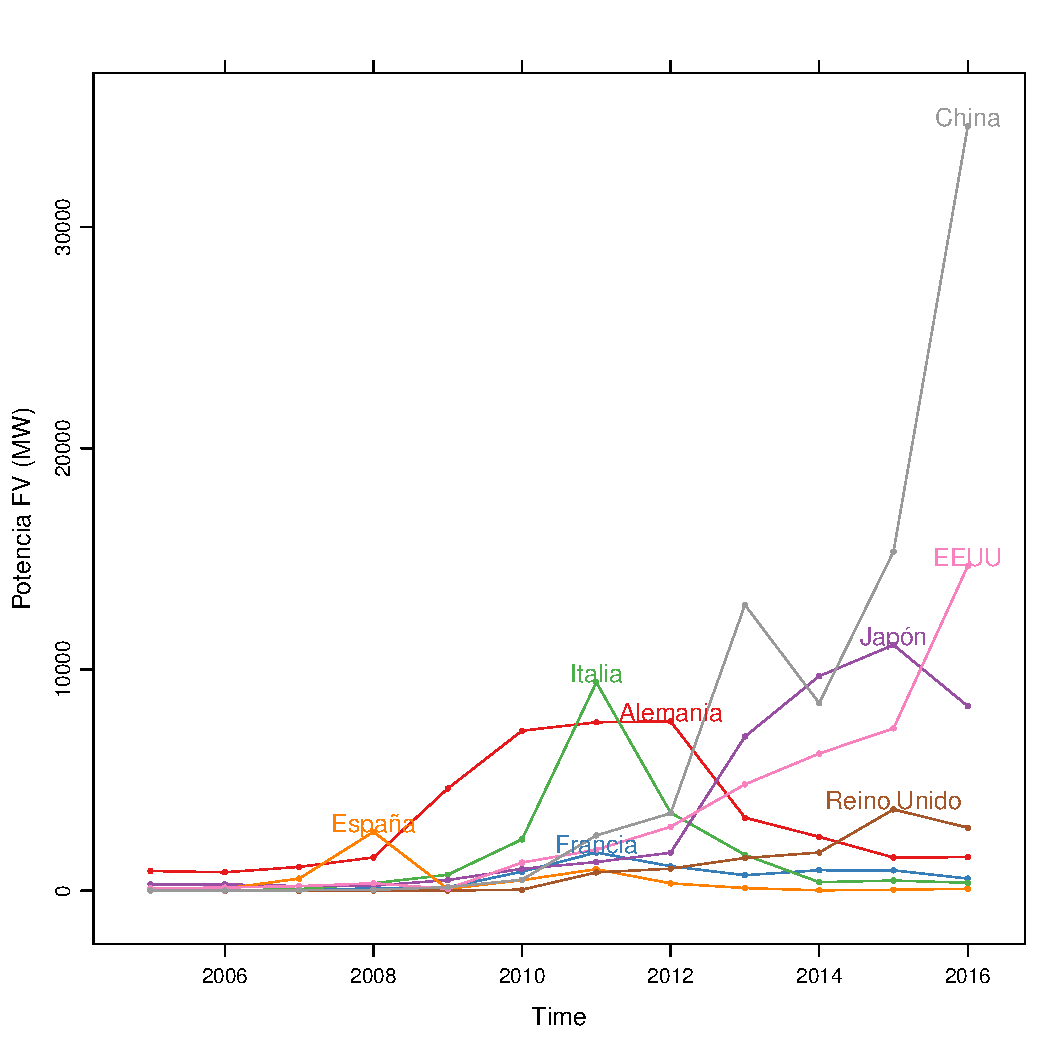
\includegraphics[width=.9\linewidth]{../figs/PVWorld.pdf}
\end{center}
\end{frame}


\begin{frame}[label={sec:org9d81681}]{Contribución energética}
\begin{block}{La ESF aporta el 2.14\% de la energía eléctrica mundial}
\begin{itemize}
\item Honduras: 13.3\%
\item Alemania: 7.47\%
\item Grecia: 7.34\%
\item Italia: 7.11\%
\item Japón: 5.93\%
\end{itemize}
\end{block}
\end{frame}

\subsection{Paridad de Red}
\label{sec:org209c9cb}

\begin{frame}[label={sec:org312437c}]{Paridad de Red}
\begin{itemize}
\item Crecimiento sostenido fuertemente relacionado con el ritmo de
reducción del precio del módulo, siendo causa y consecuencia del
mismo.

\item En estas circunstancias, los sistemas fotovoltaicos han alcanzado ya
la paridad de red en muchas partes del mundo.
\end{itemize}
\end{frame}


\begin{frame}[label={sec:org29566c4}]{}
\begin{center}
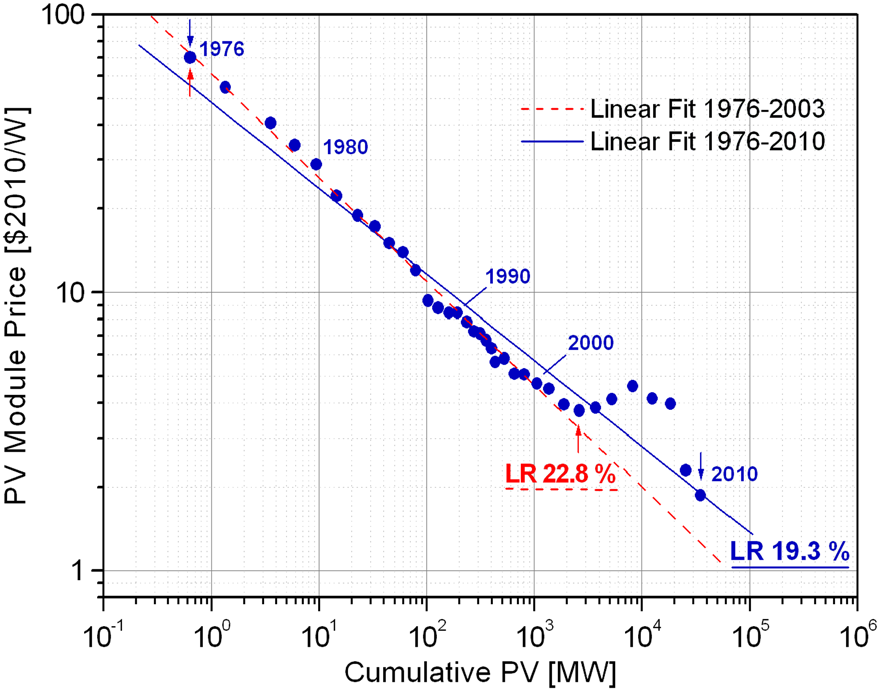
\includegraphics[width=.9\linewidth]{../figs/CurvaAprendizajeFV_BreyerPiP.png}
\end{center}
\end{frame}

\begin{frame}[label={sec:orge48c834}]{Paridad en 2010\footnote{El color naranja identifica los sistemas residenciales y el azul los
sistemas industriales. El tamaño de los círculos está relacionado con
el tamaño del mercado eléctrico de cada país.}}
\begin{center}
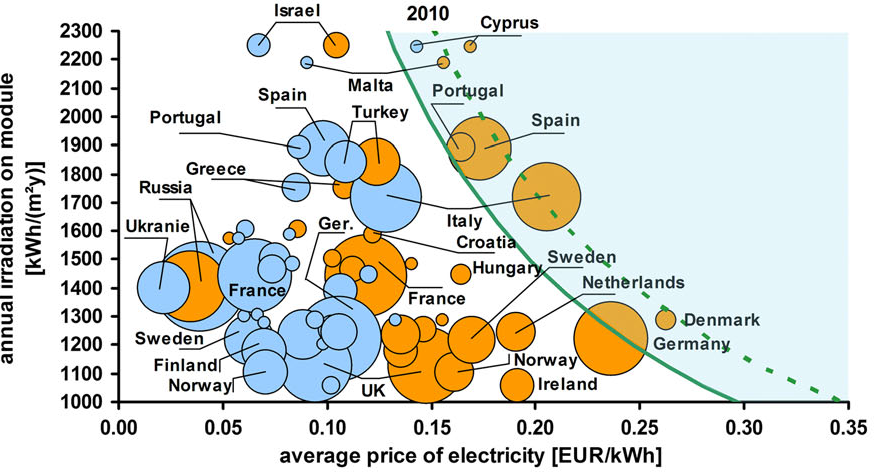
\includegraphics[width=.9\linewidth]{../figs/GridParity2010.png}
\end{center} 
\end{frame}


\begin{frame}[label={sec:orgb5a86ae}]{Paridad en 2013\footnote{El color naranja identifica los sistemas residenciales y el azul los
sistemas industriales. El tamaño de los círculos está relacionado con
el tamaño del mercado eléctrico de cada país.}}
\begin{center}
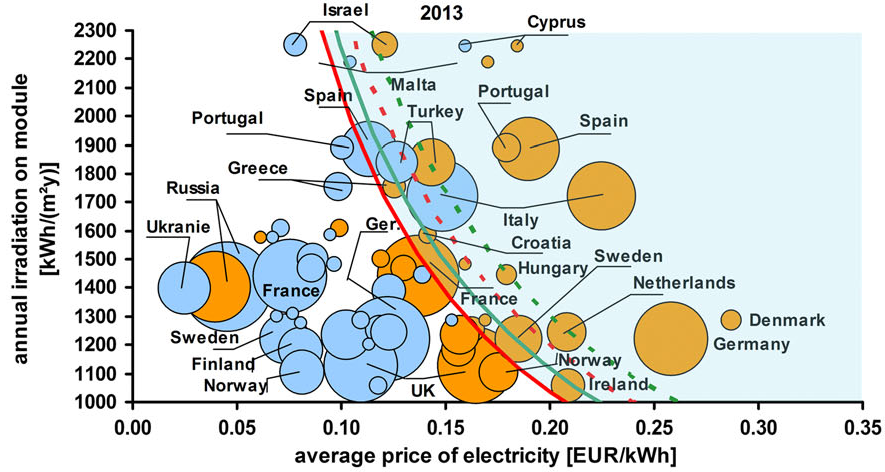
\includegraphics[width=.9\linewidth]{../figs/GridParity2013.png}
\end{center}
\end{frame}


\subsection{Segmentos de mercado}
\label{sec:org8e484e1}

\begin{frame}[label={sec:org9bad7bd}]{Segmentos de Mercado}
\begin{itemize}
\item La European Photovoltaics Industry Association diferencia entre:
\begin{itemize}
\item sistemas sobre terreno,
\item sistemas en entorno industrial,
\item comercial,
\item y residencial.
\end{itemize}
\end{itemize}

\begin{center}
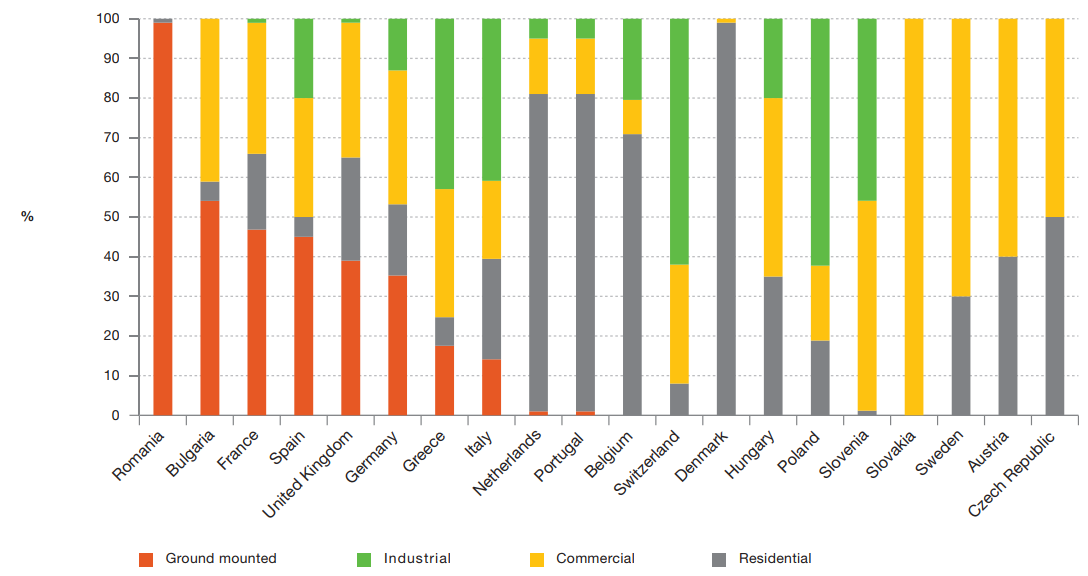
\includegraphics[width=.9\linewidth]{../figs/SegmentacionFVEuropa_EPIA.png}
\end{center}
\end{frame}

\begin{frame}[label={sec:org3d7d912}]{Segmentación en Alemania y España}
\begin{itemize}
\item El mercado fotovoltaico español se ha basado en sistemas sobre
terreno (plantas fotovoltaicas).

\item El mercado alemán ha diversificado las opciones dando mayor
preponderancia a sistemas comerciales y residenciales.
\end{itemize}
\end{frame}

\begin{frame}[label={sec:orga28a734}]{Tamaño de instalación y Conexión}
\begin{block}{España}
\begin{itemize}
\item Tamaño medio \SI{107}{\kilo\watt}

\item 64\% en redes de AT/MT.

\item 36\% en redes de BT.
\end{itemize}
\end{block}

\begin{block}{Alemania}
\begin{itemize}
\item Tamaño medio \SI{17}{\kilo\watt}

\item 38\% en redes de AT/MT

\item 62\% en redes de BT
\end{itemize}
\end{block}

\begin{block}{Japón}
\begin{itemize}
\item Tamaño medio por debajo de \SI{5}{\kilo\watt}

\item 80\% del total en BT.
\end{itemize}
\end{block}
\end{frame}
\end{document}